\section*{Questão 8}

\paragraph{} Primeiramente calculamos o protudo vetorial dado:

\begin{equation}
    (t'(s), y'(s)) \times  (t''(s), y''(s)) = (0,0,t'(s)y''(s) - y'(s)t''(s))
\end{equation}

portanto:

\begin{equation}
     \kappa(s) =  \frac{||(t'(s), y'(s)) \times  (t''(s), y''(s))||}{||(t'(s), y'(s))||^{3}} = 
     \frac{|t'(s)y''(s) - y'(s)t''(s)|}{(t'(s)^2 + y'(s)^2)^{\frac{3}{2}}}
    \label{eq:quest8}
\end{equation}

além disso as derivadas são conhecidas uma vez que já temos os coeficientes que determinam
y(s) e t(s). Basta então resolver os coeficientes e calcular a função acima com s variando de 0 a 1
em cada subintervalo. O resultado junto com o ajuste por splines e os dados tabelados são mostrados n
a figura \ref{fig:quest8}.

\paragraph{}O gráfico nos mostra, assim como a fórmula \ref{eq:quest8} já previa, que nos pontos
onde a reta tangente ao ajuste é horizontal, ou seja, quando a primeira derivada se anula, a curvatura
é infinita(limitamos os eixos para poder visualizar melhor o resultado, sem isso os elevados valores
assumidos nas singularidades não permitiriam entendimento dos resultados). Além disso, e mais interessante,
a curvatura é baixíssima na maioria dos pontos do domínio. A baixa curvatura significa que a curva é extremamente
suave. Digamos que quiséssemos criar uma animação e tivéssemos pouco poder computacional, de modo que um número
reduzido de potos a serem considerados seria vantajoso para a simulação. Nesse caso a técnica de ajuste por splines
nos permitiria integrar as posições da um número reduzido de pontos e completar a curva entre eles de forma suave.
Dessa forma teríamos uma boa representação da superfície suave de um corpo e a pouco custo computacional.

\paragraph{}É interessante notar que a curvatura nos extremos se aproxima de 0, o que decorre do fato de,
em nosso algoritmo termos imposto a condição de contorno natural Y''(0) = Y''(1) = 0.

\paragraph{}Na análise aqui apresentada o cálculo da curva de torção foi feita conhecendo-se 
os coeficientes e avaliando a função da torção em cada ponto do gráfico(a rigor, em 100 pontos entre cada
ponto tabelado). Poderíamos também calcular a curvatura apenas nos pontos tabelados e completar os intervalos
com a mesma técnica de spline utilizada. Teríamos assim uma aproximação para a torção que pode não ser a ideal
mas seria rapidamente calculada, baseada em um número reduzido de pontos(100 vezes menos que no primeiro 
método).

\FloatBarrier
\begin{figure}[!htp]
	% GNUPLOT: LaTeX picture with Postscript
\begingroup
  \fontfamily{phv}%
  \selectfont
\definecolor{t}{rgb}{0.5,0.5,0.5}
  \makeatletter
  \providecommand\color[2][]{%
    \GenericError{(gnuplot) \space\space\space\@spaces}{%
      Package color not loaded in conjunction with
      terminal option `colourtext'%
    }{See the gnuplot documentation for explanation.%
    }{Either use 'blacktext' in gnuplot or load the package
      color.sty in LaTeX.}%
    \renewcommand\color[2][]{}%
  }%
  \providecommand\includegraphics[2][]{%
    \GenericError{(gnuplot) \space\space\space\@spaces}{%
      Package graphicx or graphics not loaded%
    }{See the gnuplot documentation for explanation.%
    }{The gnuplot epslatex terminal needs graphicx.sty or graphics.sty.}%
    \renewcommand\includegraphics[2][]{}%
  }%
  \providecommand\rotatebox[2]{#2}%
  \@ifundefined{ifGPcolor}{%
    \newif\ifGPcolor
    \GPcolortrue
  }{}%
  \@ifundefined{ifGPblacktext}{%
    \newif\ifGPblacktext
    \GPblacktextfalse
  }{}%
  % define a \g@addto@macro without @ in the name:
  \let\gplgaddtomacro\g@addto@macro
  % define empty templates for all commands taking text:
  \gdef\gplbacktext{}%
  \gdef\gplfronttext{}%
  \makeatother
  \ifGPblacktext
    % no textcolor at all
    \def\colorrgb#1{}%
    \def\colorgray#1{}%
  \else
    % gray or color?
    \ifGPcolor
      \def\colorrgb#1{\color[rgb]{#1}}%
      \def\colorgray#1{\color[gray]{#1}}%
      \expandafter\def\csname LTw\endcsname{\color{white}}%
      \expandafter\def\csname LTb\endcsname{\color{black}}%
      \expandafter\def\csname LTa\endcsname{\color{black}}%
      \expandafter\def\csname LT0\endcsname{\color[rgb]{1,0,0}}%
      \expandafter\def\csname LT1\endcsname{\color[rgb]{0,1,0}}%
      \expandafter\def\csname LT2\endcsname{\color[rgb]{0,0,1}}%
      \expandafter\def\csname LT3\endcsname{\color[rgb]{1,0,1}}%
      \expandafter\def\csname LT4\endcsname{\color[rgb]{0,1,1}}%
      \expandafter\def\csname LT5\endcsname{\color[rgb]{1,1,0}}%
      \expandafter\def\csname LT6\endcsname{\color[rgb]{0,0,0}}%
      \expandafter\def\csname LT7\endcsname{\color[rgb]{1,0.3,0}}%
      \expandafter\def\csname LT8\endcsname{\color[rgb]{0.5,0.5,0.5}}%
    \else
      % gray
      \def\colorrgb#1{\color{black}}%
      \def\colorgray#1{\color[gray]{#1}}%
      \expandafter\def\csname LTw\endcsname{\color{white}}%
      \expandafter\def\csname LTb\endcsname{\color{black}}%
      \expandafter\def\csname LTa\endcsname{\color{black}}%
      \expandafter\def\csname LT0\endcsname{\color{black}}%
      \expandafter\def\csname LT1\endcsname{\color{black}}%
      \expandafter\def\csname LT2\endcsname{\color{black}}%
      \expandafter\def\csname LT3\endcsname{\color{black}}%
      \expandafter\def\csname LT4\endcsname{\color{black}}%
      \expandafter\def\csname LT5\endcsname{\color{black}}%
      \expandafter\def\csname LT6\endcsname{\color{black}}%
      \expandafter\def\csname LT7\endcsname{\color{black}}%
      \expandafter\def\csname LT8\endcsname{\color{black}}%
    \fi
  \fi
  \setlength{\unitlength}{0.0500bp}%
  \begin{picture}(7936.00,5668.00)%
    \gplgaddtomacro\gplbacktext{%
      \csname LTb\endcsname%
      \put(666,1296){\makebox(0,0)[r]{\strut{} 0}}%
      \put(666,1993){\makebox(0,0)[r]{\strut{} 2}}%
      \put(666,2689){\makebox(0,0)[r]{\strut{} 4}}%
      \put(666,3386){\makebox(0,0)[r]{\strut{} 6}}%
      \put(666,4082){\makebox(0,0)[r]{\strut{} 8}}%
      \put(666,4779){\makebox(0,0)[r]{\strut{} 10}}%
      \put(774,1116){\makebox(0,0){\strut{} 0}}%
      \put(1534,1116){\makebox(0,0){\strut{} 0.2}}%
      \put(2293,1116){\makebox(0,0){\strut{} 0.4}}%
      \put(3053,1116){\makebox(0,0){\strut{} 0.6}}%
      \put(3813,1116){\makebox(0,0){\strut{} 0.8}}%
      \put(4572,1116){\makebox(0,0){\strut{} 1}}%
      \put(5332,1116){\makebox(0,0){\strut{} 1.2}}%
      \put(6092,1116){\makebox(0,0){\strut{} 1.4}}%
      \put(6851,1116){\makebox(0,0){\strut{} 1.6}}%
      \put(7611,1116){\makebox(0,0){\strut{} 1.8}}%
      \put(144,3211){\makebox(0,0){\strut{}$\kappa(t)$}}%
      \put(4192,846){\makebox(0,0){\strut{}t}}%
      \put(4192,5397){\makebox(0,0){\strut{}Curvatura do ajuste com splines}}%
    }%
    \gplgaddtomacro\gplfronttext{%
      \csname LTb\endcsname%
      \put(4431,513){\makebox(0,0)[r]{\strut{}$\kappa (t)$}}%
      \csname LTb\endcsname%
      \put(4431,333){\makebox(0,0)[r]{\strut{}splines}}%
      \csname LTb\endcsname%
      \put(4431,153){\makebox(0,0)[r]{\strut{}data points}}%
    }%
    \gplbacktext
    \put(0,0){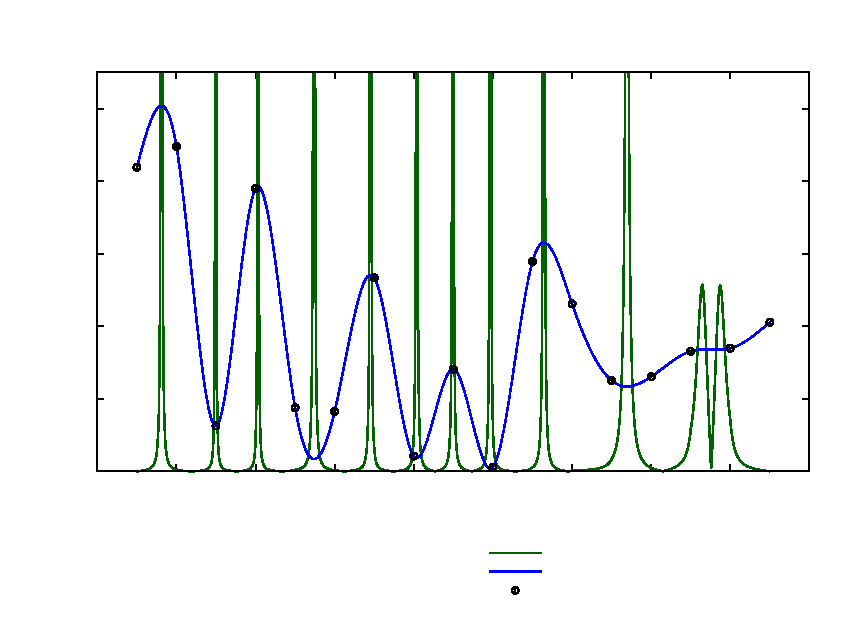
\includegraphics{./../LaTeX/graph/quest8}}%
    \gplfronttext
  \end{picture}%
\endgroup

	\caption{Curvatura da interpolação com splines}
	\label{fig:quest8}
\end{figure}
\FloatBarrier
